\section{Auswertung}
\label{sec:Auswertung}


\subsection{Blockschaltbild}
\subsection{Grafische Darstellung der Stackspannung, der
Stackleistung, der Verbraucherleistung und des Wasserstoffverbrauchs}
\begin{figure}[H]
    \centering
    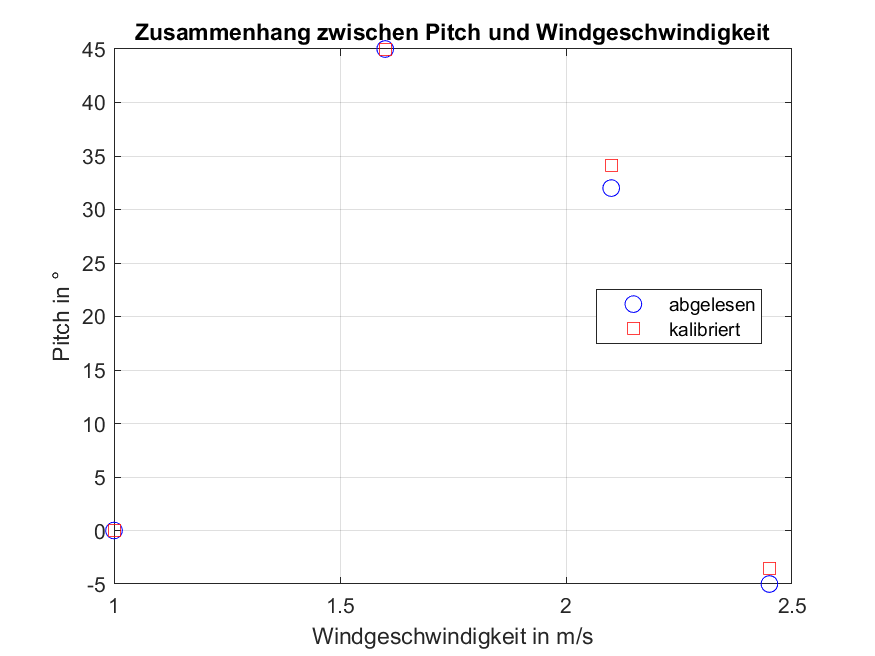
\includegraphics[width=0.8\textwidth]{plot1}
    \caption{Grafische Darstellung der Stackspannung, der
    Stackleistung, der Verbraucherleistung und des Wasserstoffverbrauchs.}
    \label{fig:plot1_26062023}
  \end{figure}
\subsection{Grafische Darstellung einiger Messgrößen im Bezug zum Verbracuherstrom}
\begin{figure}[H]
    \centering
    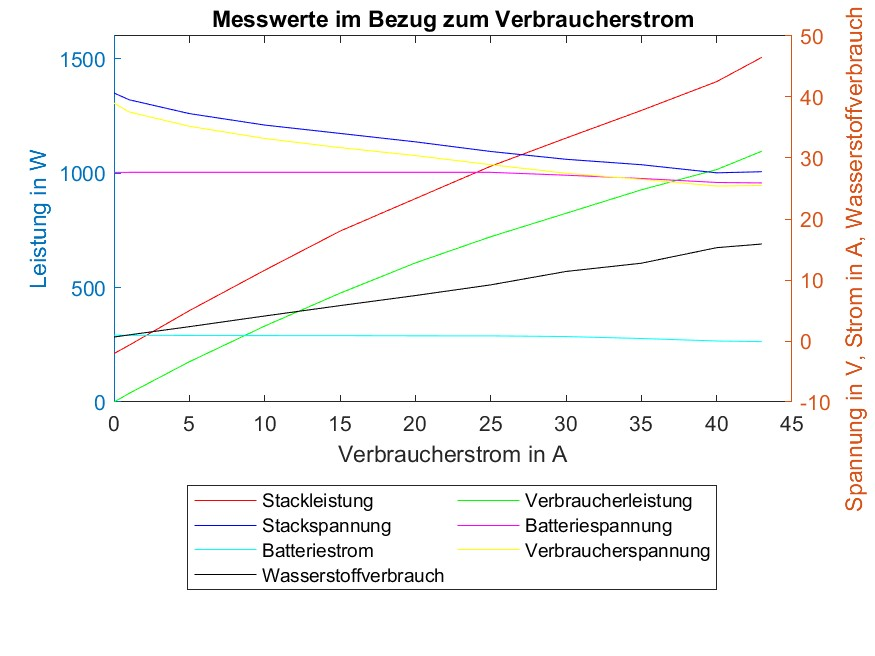
\includegraphics[width=0.8\textwidth]{grafik2}
    \caption{Grafische Darstellung der Stackspannung, der
    Stackleistung, der Verbraucherleistung und des Wasserstoffverbrauchs.}
    \label{fig:plot2_26062023}
  \end{figure}
  Um nun im nächsten Schritt den Wirkungsgrad des Stacks anhand des Heiz- und Brennwertes zu bestimmen muss man den Wasserstoffverbrauch mit Hilfe des Heizwertes von $3 \frac{kWh}{m^3}$ und des Brennwerts von $3,54 \frac{kWh}{m^3}$
von Wasserstoff kann unser Wasserstoff Verbrauch nun in eine Leistung umgerechnet werden. Die tatsächlichen Leistungen an Stack und Gesamtsystem werden nun durch die vorher berechnete Leistung geteilt. Die folgende Gleichung zeigt diese Beispielhaft für den Stackwirkungsgrad:
\begin{equation}
 \eta= \frac{P_{Stack}}{H2_{Verbrauch_Stack}*H2_{Brennwert}}= \frac{1,506 kWh}{3,54 \frac{kWh}{m^3 }\cdot 0,954 \frac{m^3}{h}}=0,45
  \label{eq:230627_Beispiel_wirkungsgrad_Berechnung}
\end{equation}
\begin{figure}[H]
    \centering
    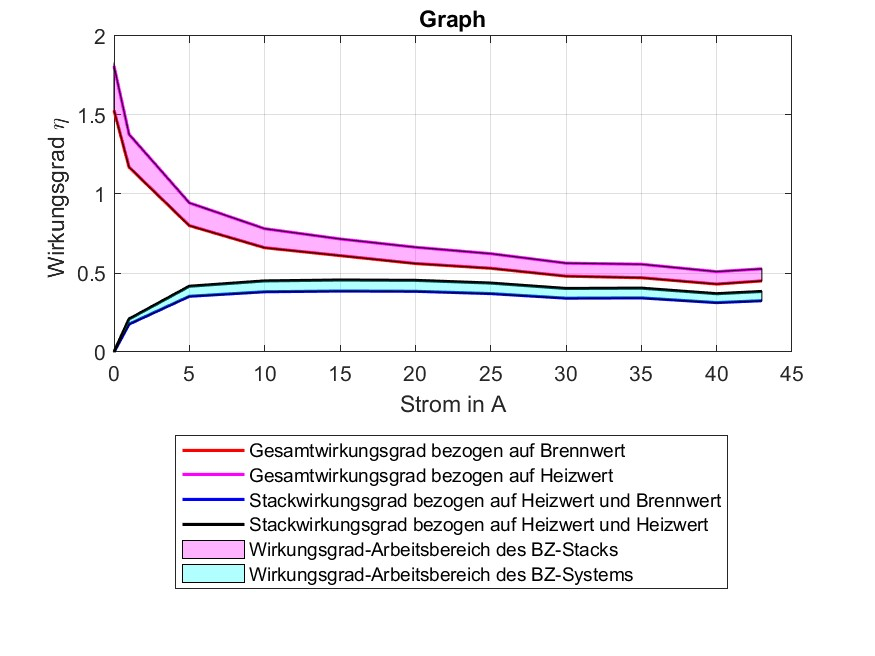
\includegraphics[width=0.8\textwidth]{plot3}
    \caption{Wirkungsgradverlauf für den Stack und das gesamte System.}
    \label{fig:plot3_26062023}
  \end{figure}
  Dabei entstehen die Wirkungsgradbänder bei Brennstoffzellen aufgrund von Verlusten in den Reaktionskinetiken, ohmschen Verlusten, Massentransportverlusten und den Betriebsbedingungen. Diese Faktoren beeinflussen die Leistungsfähigkeit und den Wirkungsgrad des Systems.
   Die Art der Brennstoffzelle und die verwendeten Materialien spielen eine Rolle bei der Ausprägung der Wirkungsgradbänder. Unterschiedliche Betriebsparameter können zu variierenden Wirkungsgradbändern führen. Es gibt verschiedene Arten von Brennstoffzellen mit jeweils spezifischen Charakteristika und Herausforderungen im Hinblick auf Wirkungsgradbänder.
   \subsection{Diskussion der Kurven}
   \autoref{fig:plot1_26062023} und \autoref{fig:plot2_26062023} zeigt die unterschiedlichen Systemspannungen in Abhängigkeit des
Verbraucherstrom und des Stack Stroms. Zu erkennen ist die charakteristische Brennstoffzellen Spannungskennlinie
 (blau in \autoref{fig:plot2_26062023} und grau in  \autoref{fig:plot1_26062023}), die in \autoref{fig:plot2_26062023} genauer beschrieben wird. Die Stack- als auch die Verbraucherleistung
steigen in Abhängigkeit des zugeführten Wasserstoffes proportional an. In den \autoref{fig:plot1_26062023} 
und \autoref{fig:plot2_26062023} ist weiterhin zu erkennen, dass bei
 steigendem Strom, sowohl die Stack- als
auch die Verbraucherspannung leicht, absinken. Die lässt sich auch an dem Abfallen des
Wirkungsgrades ablesen.
\\ In \autoref{fig:plot3_26062023} ist der Verlauf des Wirkungsgrads des Stacks (schwarz und blau) sowie des Gesamtwirkungsgrads (rot und magenta) dargestellt. Der Wirkungsgrad wurde jeweils unter Verwendung des oberen und unteren Heizwerts berechnet, und die Toleranzbänder sind farblich gekennzeichnet. Es ist zu beachten, dass der Wirkungsgrad des Stacks deutlich über 100 Prozent liegt, was eigentlich nicht möglich ist und im krassen Gegensatz zum Verlauf des Gesamtwirkungsgrads steht.
Der Grund dafür liegt darin, dass die Brennstoffzelle bei Inbetriebnahme die Membranen spült, um sie von Unreinheiten und Ablagerungen zu befreien. Dieses Spülen der Membranen erfolgt mit Wasserstoff, wodurch für einen bestimmten Zeitraum deutlich mehr Wasserstoff zur Verfügung steht. Dadurch beginnt die Zellreaktion, bevor eine Leistungsabnahme des Verbrauchers eintritt. Dies führt zu den beschriebenen Wirkungsgraden des Stacks, die während des Startvorgangs über 1 liegen.
\\
\subsection{}
\subsection{Teillastverhalten}

Die Brennstoffzelle hat einen sehr guten Teillastwirkungsgrad. In der zweiten Teillast-Messung ist die Brennstoffzelle wärmer als zuvor und hat ihre optimale Betriebstemperatur erreicht. Die Bauteile der Schaltung (Kompressor und Kühlung) sind eingeschwungen. Es werden bessere Werte als in der ersten Messung bei 20A erreicht. Außerdem auffällig ist der hohe Batteriestrom, dieser ist so hoch, da die Batterie vorher (durch hohe Lastströme) entladen und nun wieder aufgeladen wird. 



\subsection{Energiebilanz für den Teillastfall}

\textbf{Messwerte noch ins Protokoll}